\section{Introduction}
\vspace{-1mm}
% Large Language Models (LLMs), empowered by strong cognitive awareness, semantic abstraction, and generative reasoning, have been widely integrated into diverse interactive workflows and agent-like application paradigms, fueling the sustained pursuit of general-purpose models' capabilities \citep{vaswani2017attention,yao2022react,schick2023toolformer,wang2024survey}. 
% In contrast, as deployment becomes increasingly fine-grained, \emph{specialized and deployable} model instances that prioritize privacy preservation, response efficiency, and controllability %as first-class requirements 
% are more likely to dominate future practical application stacks~\citep{belcak2025slmfuture,belcak2025nvidiaslmblog}. 
% This gap is amplified by the heterogeneous and long-tailed nature of deployment scenarios, where high-quality task data and sustained optimization pipelines are often unavailable or prohibitively expensive~\citep{kaplan2020scaling}. 
% These constraints motivate \emph{post-training specialization} via compression under post-training and data-scarce regimes: extracting high capability-density and budget-bounded compressed instances from a general LLM base to improve deployability, generalization, and reuse under strict inference constraints~\citep{han2016deepcompression,frankle2019lottery,wan2023efficientllm_survey}.

Large Language Models (LLMs) are becoming the core engines behind modern intelligent applications with strong reasoning and generative capabilities~\cite{vaswani2017attention,yao2022react,schick2023toolformer,wang2024survey}. 
% However, as LLM-powered systems mature, practitioners increasingly recognize that a single general-purpose model is not always the most effective deployment choice. 
%As real-world applications become increasingly specialized, domain-specific LLMs are essential for scenarios requiring repeated invocations within a consistent context ~\cite{belcak2025slmfuture,belcak2025nvidiaslmblog}.
As these real-world applications become increasingly dedicated, specialized LLMs are typically required in specific scenarios~(where models is repeatedly invoked within coherent contexts)~\cite{belcak2025slmfuture,belcak2025nvidiaslmblog}.
%to execute relatively vertical tasks.
%, pushing deployments toward finer-grained, on-device, and resource-constrained settings. 
However, scenario-specific LLM is substantially constrained by the heterogeneous and long-tailed nature of real-world application scenarios, where high-quality scenario-specific training data and optimization pipelines are often unavailable or prohibitively expensive~\cite{kaplan2020scaling}. 
%while delivering substantially improved inference efficiency?

\begin{figure}[t]
\centering
  % \begin{flushright}
    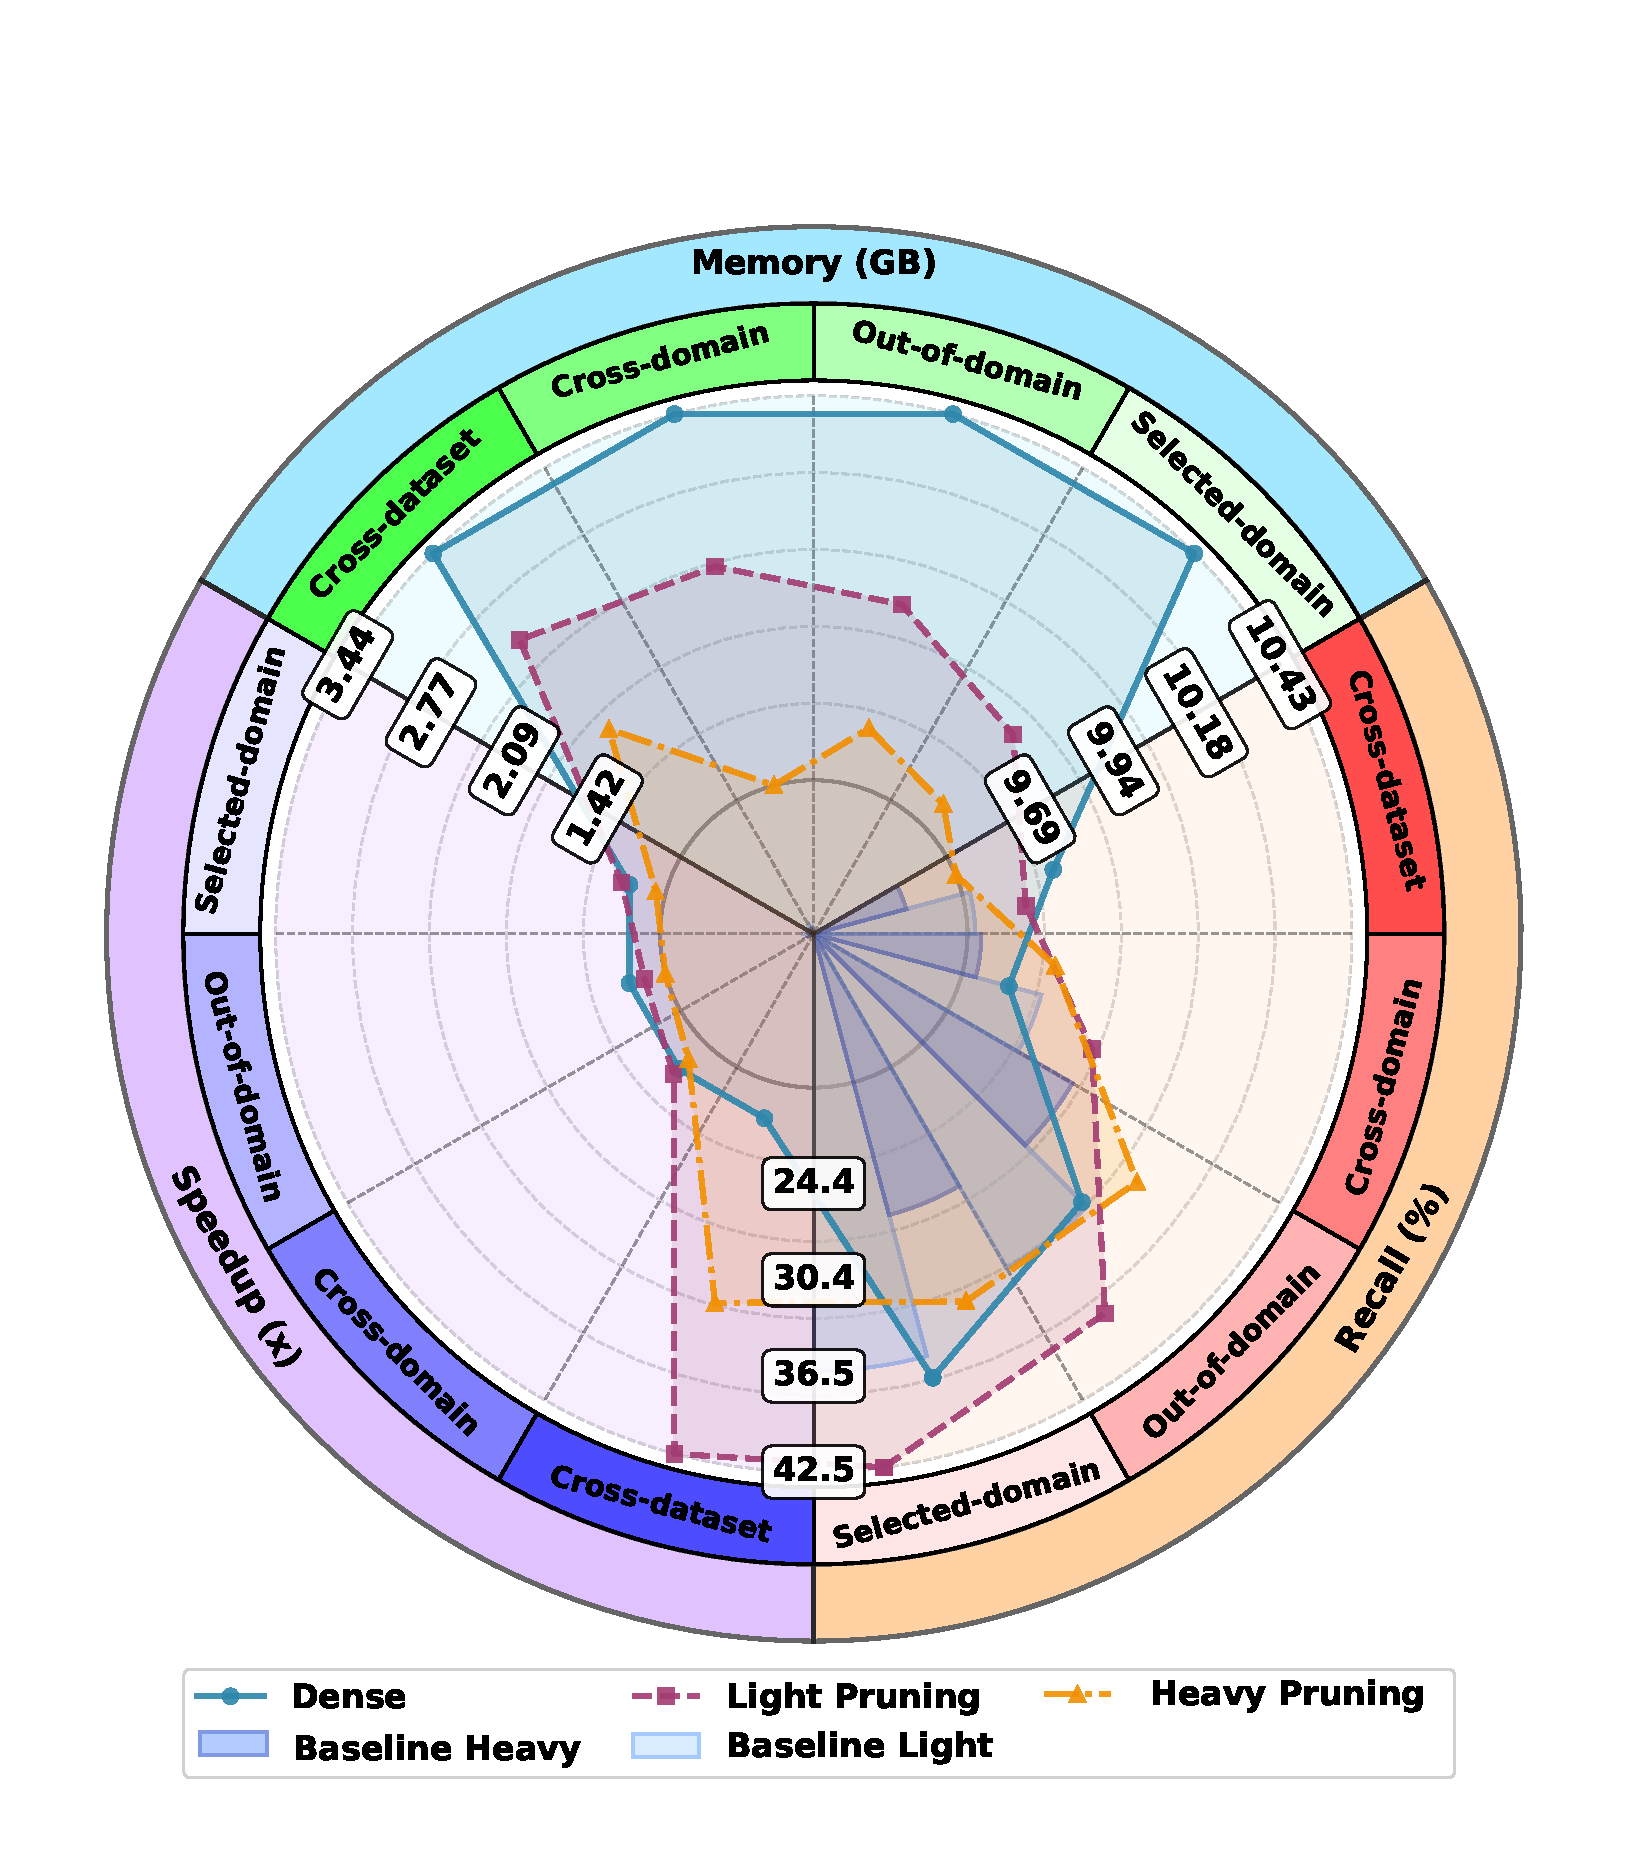
\includegraphics[width=0.46\textwidth]{figs/radar_average.pdf}
  % \end{flushright}
  \vspace{-1mm}
  \caption{\textbf{Model-average radar chart} demonstrates the robustness of  \textsc{SubspacePath Pruner} across various domains and datasets with individual models behavior provided in Figure~\ref{fig:radar_charts_all}.}
  %\vspace{-1mm}
  \label{fig:radar_average_intro}
\end{figure}


% % Nonetheless, existing specialization methods exhibit clear gaps. Training-based approaches (e.g., fine-tuning and distillation) inherently rely on data availability and training pipelines \citep{hu2021lora,hinton2015distilling}; inference-time approaches (e.g., retrieval-augmented generation (RAG) and long-context prompting) introduce latency and stability issues while shifting adaptation costs to online inference \citep{lewis2020rag,dai2019transformerxl,beltagy2020longformer}. Mixture-of-Experts (MoE) for specialized scenarios still incur large total parameter counts and training dependencies, inevitably have high deployment and maintenance costs \citep{shazeer2017outrageously,fedus2021switch}. 

% However, existing specialization paradigms exhibit persistent gaps under practical constraints. Training-based adaptation and inference-time mechanisms incur nontrivial data, optimization, or deployment overheads and can degrade in stability and generalization~\citep{hu2021lora,hinton2015distilling,lewis2020rag,dai2019transformerxl,beltagy2020longformer,shazeer2017outrageously}. 
% Moreover, existing model compression techniques still lack reliable robustness guarantees~\citep{yuan2023revisitingoodnlp,yang2024advoodrobustness}. 
% Budget-constrained pruning typically relies on global or average static importance, which can induce inference sensitivity and brittle behavior under distribution shifts~\citep{michel2019sixteen,frantar2023sparsegpt,sun2023wanda,lele2025rethinking_tfsp}. 
% Structured routing (e.g., MoE-style routing or rule-/router-driven pruning) can improve specialization but remains sensitive to router mis-specification and distribution mismatch, especially under personalization and shift~\citep{hou2025instructionfollowing,dong2024griffin,wee2025pudding}. 

\begin{figure*}[!t]
  \centering
  
\includegraphics[width=0.92\textwidth]{figs/main.pdf}
  \vspace{-1mm}
  \caption{\textbf{Overview of \textsc{SubspacePath Pruner}.} \ding{172}\textbf{DBS} defines a stable basis of domain axes in embedding space, and \textbf{PSP} \ding{173}trains a lightweight \emph{probe} with head importance and whitelist cached and \ding{174}uses probe to couple axes to sparse internal head pathways.}
  \label{fig:at_a_glance}
\end{figure*}

Motivated by these constraints, \emph{post-training specialization}~\cite{frankle2019lottery,wan2023efficientllm_survey} has emerged as a practical method for deriving inference instances in data-scarce and budget-limited settings.
Compared with conventional specialization methods requiring additional training (e.g., fine-tuning, distillation) or inference-time adaptation (e.g., retrieval augmentation, long-context prompting), which introduce complexity and high cost in practical inference~\cite{hu2022lora,hinton2015distilling,lewis2020rag,dai2019transformerxl,beltagy2020longformer,shazeer2017outrageously}, post-training specialization produces model instances \emph{practically} via \emph{inference-time computing} applied after pretraining.
% Conventional specialization methods, such as fine-tuning or distillation, often entail high computational costs and complex inference-time adaptations (e.g., RAG or long-context prompting) \cite{hu2022lora, hinton2015distilling, lewis2020rag}. To address these constraints, \textit{post-training specialization} \cite{frankle2019lottery, wan2023efficientllm_survey} has emerged as a more practical alternative. It enables the derivation of efficient inference instances specifically for data-scarce and budget-limited settings without the overhead of additional training.
Specifically, existing post-training specialization methods are primarily built upon \emph{model compression}~\cite{yuan2023revisitingoodnlp,yang2024advoodrobustness}, with \emph{budget-constrained pruning} or \emph{structured cache routing} mechanisms (e.g., MoE-style router-based pruning)  being representative instantiations~\cite{hou2025instructionfollowing,dong2024griffin,wee2025pudding}. 
However, these approaches still exhibit persistent gaps under practical constraints. 
First, compression methods~\cite{michel2019sixteen,frantar2023sparsegpt, sun2023wanda,lele2025rethinking_tfsp} often rely on global or average static importance criteria, which induce sensitivity and brittle behavior across diverse scenarios. 
Second, structured cache routing heavily depends on router design and calibration, making it vulnerable to router mis-specification and scenario mismatch. Therefore, these limitations raise a question: \emph{Can we practically and robustly extract scenario-specific instances from an LLM base without extra scenario-specific training data while preserving the capability of inference?}
%Therefore, in \emph{inference-time} setting, we need to focus on designing a pruning mechanism that remains robust across various heterogeneous scenarios.
%from the labeling space used by routers or probes, namely under \emph{out-of-distribution} mismatch.

To address this, we investigate the internal space of LLMs and identify a consistent structural regularity: \emph{representation-subspaces (e.g., domains) in embedding-space are coupled with sparse internal reasoning parameter-pathways in model-space.}%
\footnote{\emph{Subspaces} refer to domain representation sets in embedding space (usually aligned with similar scenarios), and \emph{pathways} denote component selection (e.g., head-wise pathways), while \emph{subnetworks} referred generically to pruned model instances.}
% Specifically, semantic variation in the \emph{input embedding space} can be characterized by a set of quasi-orthogonal \emph{domain axes}, and each axis tends to repeatedly activate only a small subset of head-wise computation pathways in the LLM. 
% This suggests that high-capability-density computation is concentrated in sparse and stable pathway sets, rather than being uniformly distributed across the full model.
% Second, these pathway sets are partially separable across reused axes, implying that a deployable subnetwork can be obtained by preserving the pathways most relevant to the target deployment domain while pruning redundant capacity.
Specifically, (i) for each quasi-orthogonal domain subspace, only a subset of head-wise computation pathways is repeatedly activated, suggesting a stable pathway set. And (ii) these pathway sets are partially separable across domains, motivating a \emph{probe-based coupling} mechanism that produces interpretable and reliable pathways for robust pruning~\cite{tenenbaum2000isomap,yao2024gpruner,gao2024sae_scaling}. 
%This resonates with evidence on sparse circuits in LLMs~\citep{gao2025weight,openai2025sparsecircuitsblog} and sparse coding or chain-like pathways in neuroscience~\citep{olshausen1996sparse,diesmann1999synfire}. 
Driven by these observations, we establish a pragmatic principle to guide the design of our method:
instead of optimizing compression ratios alone, we should preserve \emph{scenario-related key pathways} and remove redundancy~\cite{zhang2024structuredpruning_llm,he2025olica}.

We propose a scenario-specific structued pruning framework, \textsc{SubspacePath Pruner}, at \emph{inference-time} as shown in Figure~\ref{fig:at_a_glance}. 
This framework provides an interpretable pruning pipeline that operates within the inference budget by explicitly coupling representation subspaces with reasoning pathways. It consists of two core components:
\begin{itemize}[parsep=0pt]
    \vspace{-2pt}
    \item \textbf{Domain-Basis Synthesis (DBS)}: \ding{172} a quasi-orthogonal basis of domain axes in embedding-space which provides a stable coordinate system for subsequent pathway scoring and selection.
    \item \textbf{Probe-based Scenario Pruning (PSP)}: \ding{173} efficient layer-wise probes \cite{alain2016linearprobes} trained to evaluate \emph{subspace$\rightarrow$pathway} coupling with whitelists. \ding{174}For specific scenarios, we compile budgeted head-wise \emph{pathway}, yielding executable pruned subnetworks practically.
\end{itemize}
\vspace{-0.5mm}
 
Experiments across 4 models and 6 dataset splits as shown in Figure~\ref{fig:radar_average_intro} show that \textsc{SubspacePath Pruner} achieves \textbf{35.8} / \textbf{25.5} Recall on cross-domain / cross-dataset tests (vs. 30.5 / 24.3 dense) at \textbf{15--20\%} pruning ratio, and \textbf{29.8} / \textbf{21.6} with up to \textbf{1.76$\times$} speedup at \textbf{25--30\%} pruning ratio.
\vspace{-0.5mm}